
\documentclass[letterpaper,12pt]{article} 

\usepackage[utf8]{inputenc}
\usepackage[spanish]{babel}
\usepackage{amsmath}
\usepackage{amsfonts}
\usepackage{amssymb} 
\usepackage{algorithm2e}
\usepackage{algorithm}
\usepackage{algorithmic}
\usepackage{graphicx} 			%graficos
\usepackage[colorlinks=true, linkcolor=black, citecolor=black, urlcolor=blue]{hyperref} 	
\usepackage{wrapfig}
\usepackage{enumitem}
\usepackage{fancyhdr}
\usepackage{float}
\usepackage{eurosym}
\usepackage{color}
\usepackage{titling}
\usepackage{lipsum}
\usepackage{tocbibind}
\usepackage{longtable,multirow,booktabs}
\usepackage{multicol}

\usepackage[left=3cm,right=3cm,top=3cm,bottom=4cm]{geometry}		%margenes para documento


\pagestyle{fancy}													% estilo del estlo de pie cabezera


%%% Para las cabeceras
\newcommand{\hsp}{\hspace{20pt}}
\newcommand{\HRule}{\rule{\linewidth}{0.5mm}}
\headheight=50pt


\newcommand{\vacio}{\textcolor{white}{holacaracola}} 			%comando para dar un texto 

% Color azul para algunos 
% textos de la portada
\definecolor{azulportada}{rgb}{0.16, 0.32, 0.75}				%color azul para una ciertas letras


%%%% Azul para textos de headings
\definecolor{azulinterior}{rgb}{0.0, 0.2, 0.6}

%====================================Datos del proyecto ======================================

%titulo del proyecto
\title{Sistema de Monitoreo y Control de Robot}				

%%%% AUTOR
\author{Mamani Yucra Alexander\\ \vspace{0.3cm}Mamani Yucra Alexander\\ \vspace{0.3cm}Mamani Yucra Alexander}

%%%%%% DIRECTOR DEL TRABAJO
\newcommand{\director}{Lic. Yony Richard Montoya Burgos}



\begin{document}

\begin{titlepage} 
\newgeometry{left=0.6cm,top=1cm,bottom=1.2cm}
\fbox{\parbox[c]{18.5cm}{  												%margen de la caratula 
\begin{center}
\vspace{1.5cm}
{\fontfamily{phv}\fontsize{20}{5}\selectfont{\textbf{UNIVERSIDAD MAYOR DE SAN SIMON}}}\\	
[2em]

{\fontfamily{phv}\fontsize{16}{4}\selectfont{\textbf{FACULTAD DE CIENCIAS Y TECNOLOGIA}}}\\	
[4em]

%importamos una imagen

\includegraphics[width=5.5cm]{images/umss.png}								
\\[1cm]

%titulo de la portada
{\fontfamily{phv}\fontsize{16}{4}\selectfont{TRABAJO DE INVESTIGACIÓN}}\\[1cm]

%\textcolor{azulportada}

{\fontfamily{phv}\fontsize{20}{5}\selectfont{\textsc{\thetitle}}}\\
[2cm]

Presentado por :
\vspace{0.5cm}

\begin{minipage}[b]{6cm}
	\begin{center}
		Univ. Alexander Mamani Y.\\
		FCyT\\
		Cocambamba\\
		akeymy4@gmail.com
	\end{center}
\end{minipage} \hfill \begin{minipage}[b]{6cm}
	\begin{center}
		Univ. Adan F. Toledo\\
		FCyT\\
		Cocambamba\\
		AdanT5@gmail.com
	\end{center}
\end{minipage} \hfill \begin{minipage}[b]{6cm}
	\begin{center}
		Univ. Juan C. Veizaga\\
		FCyT\\
		Cocambamba\\
		carlos12@gmail.com 
	\end{center}

\end{minipage}\\
[0.9cm]
{\fontfamily{phv}\fontsize{12}{3}\selectfont{Director :}}\\
[0.5cm]
{\fontfamily{phv}\fontsize{12}{3}\selectfont{\director}}\\
[2cm]
{\fontfamily{phv}\fontsize{12}{3}\selectfont{Cochabamba, 2018}}\\[1cm]
\end{center}

}}
 
 
% =============================empezamos a redactar el texto=================

 \restoregeometry  					% Volvemos a la estructura de la página normal

\end{titlepage}



{%\Large

\newpage

%%%Encabezamiento y pie de página
%%% También se genera automáticamente
%%% Mejor no tocarlo mucho.
\renewcommand{\headrulewidth}{0.5pt}
\fancyhead[R]{
	\textcolor{azulinterior}{\fontfamily{phv}\fontsize{14}{4}\selectfont{\textbf{\thetitle}}}\\
\textcolor{azulportada}{\fontfamily{phv}\fontsize{10}{3}\selectfont{Proyecto de investigación de la UMMS --  mayo-2018}}\\
}
\fancyhead[L]{\vacio}

%=================================pie de pagina==========================
\renewcommand{\footrulewidth}{0.5pt}
\fancyfoot[L]{\footnotesize Sistema de Monitoreo y Control de Robot--FCyT--- mayo-2018}
\fancyfoot[C]{\vacio}														%hacemos uso del comando que creamo \vacio
\fancyfoot[R]{\footnotesize Página \thepage}								%numeracion de la pagina					
\
\vacio
\

\vspace{1cm}
\begin{minipage}[b]{5.3cm}
	\begin{center}
		Univ. Alexander Mamani Y.\\
		FCyT\\
		Cochabamba\\
		akeymy4@gmail.com
	\end{center}
\end{minipage} \hfill \begin{minipage}[b]{4cm}
	\begin{center}
		Univ. Adan F. Toledo\\
		FCyT\\
		Cochabamba\\
		AdanT5@gmail.com
	\end{center}
\end{minipage} \hfill \begin{minipage}[b]{4.5cm}
	\begin{center}
		Univ. Juan C. Veizaga\\
		FCyT\\
		Cochabamba\\
		carlos12@gmail.com
	\end{center}
\end{minipage}

\vspace{2cm}

\subsection*{Resumen}
	Los vehículos no tripulados terrestres han demostrado que tienen múltiples usos según el concepto que se les de, dichos usos pueden ser beneficiosos para la sociedad buscando la mejoría de su calidad de vida, pero como siempre es muy difícil que todo sea bueno, y así como hay impactos positivos los hay negativos.\\
	
	Estos vehículos no tripulados se están empleando en el sector portuario para realizar tareas de mantenimiento, seguridad, gestión del tráfico y control del transporte de mercancías entre otras labores. La reducción de costes es una de sus ventajas ya que elimina los accidentes y mejora los procesos al poder actuar de forma autónoma y sin poner en riesgo a los trabajadores.\\
	
	Entoces podemos apreciar la gran importacia de estos tipos de vehiculos no tripulados.\\
	
	En el presente trabajo se pretende implementar un Software de que nos permita manejar, monitorear y mostrar datos estadisticos de un vehiculo terrestre no tripulado, mediante una interfaz grafica que facilite al usuario el manejo del mismo, asi tambien describiremos cada modulo del software y patrones de diseño  utilizados para su creacion y posterior implementacion
	
	

\vspace{1cm}
\ %% Así hago que se abra más espacio entre renglones.

\
\hrule
\
\

\paragraph{Palabras clave:} Dron terrestre, Arduino, Sistema de manejo y monitoreo de dron terrestre.

\
\newpage
\tableofcontents
\newpage



\section{INTRODUCCIÓN}
\vspace{1.5cm}

Arduino es una compañía open source y open hardware, así como un proyecto y comunidad internacional que diseña y manufactura placas de desarrollo de hardware para construir dispositivos digitales y dispositivos interactivos que puedan sensar y controlar objetos del mundo real.
Arduino se enfoca en acercar y facilitar el uso de la electrónica y programación de sistemas embebidos en proyectos multidisciplinarios.

Teniedo en cuenta los problemas plantenados con que cuenta nuestra sociedad como ser el sector portuario, y entre otros.

Se pretemde desarrollar modulos que nos permitan manipular el hardware de un dron terrestre, como asi tambien monitorear y extraer datos extadisticos del  mismo, para despues implementar en un Robot que tiene como microcontrolador Arduino.

La manipulacion de estos modulos se llevara acabo atravez de una interfaz Grafica, que reaccionara a ciertos eventos.

El Robot(hardware), cuenta con 3 Servo Motores dos para las ruedas y una para una pinza que nos permite agarrar objetos, además de un modulo bluetooth que nos permitira la transmisión y recepción de datos,un sensor ultrasonido que es usado para medir la distacia entre el Robot y un objeto.

Las tecnologias usadas para el desarrollo e implementacion del proyecto son las siguiente:

\begin{itemize}
	\item como Lenguaje de Programacion se uso Python en su version 3.
	
	\item como almacenamiento de datos se uso la estructura XML.
		
\end{itemize}


\section{DISEÑO DEL SOFTWARE}


\subsection{Arquitectura}
	
	Como base para la desarrolo del software se uso la Arquitectura de software MVC, ya que el mismo nos permite serarar el modelo de datos del software de la interfaz grafica del usuario, asi mismo nos ayudo a la mejor estructuracion del sofware y a ser mas escalable al momento de implementar nuevas funcionalidades\\

Los modulos que se desarrollados se encuentran en los siguientes paquetes:
\begin{itemize}
	\item \textbf{View.- } Paquete que contiene modulos que nos permitiran manipular la interfaz grafica de nuestro Software, separando la interfaz del usuario con el modelo del negocio
	
	\item \textbf{Controller.- }Paquete que contiene modulos que nos permitiran capturar los eventos producidos en nuestro View, y en base a estos desencadenar acciones que seran reflejadas en nuestra Interfaz Grafica
		
	\item \textbf{Model.- }Paquete que contiene modulos que nos permitiran manipular los datos generados por nuetro software, como ser guardar los datos al momento en que se graba una movimiento del Robot
	
\end{itemize}

%\begin{figure}[h]
%	\centering
%	\begin{minipage}[t]{5.5cm}
%		\includegraphics[width=5.5cm]{grafico1.png}	 %importamos una imagen
%		\caption{ Funcionamiento de un sistema de control de	versiones}		
%	\end{minipage}	
%\end{figure}

\subsection{View}
En este Paquete se encuentrar los modulos encargados de manejar la interfaz grafica, con la cual un Usuario cualquiera podra interactuar de manera intuitiva con nuestro software.

Este paquete cuenta con las siguientes clases :\\
\begin{itemize}
	\item \textbf{Ventana.- }Clase que se encargar de graficar todos los componentes de la interfaz grafica como ser: label, botones, Robot,.. etc
	
	\item \textbf{Robot.- }Clase Singleton que nos permite dibujar en la Ventana todos los comportamientos del robot como ser Avanzar, Retroceder, girar a la izquierda, girar a la derecha, Detener, abrir y cerrar pinza
	
	\item \textbf{Grafica.- }Clase que despliega distintos tipos de graficos estadisticos , con los datos proporcionados por la Clase Model.Estadistica.
	
\end{itemize}


\subsection{Controller}
En este Paquete se encuentrar los modulos encargados de capturar los eventos producidos en el View, y en base a estos realizar una accion, ya sea de grabar o reproducir un accion previemente grabada.\\

Este paquete cuenta con las siguientes clases y modulos :
	\begin{itemize}
		\item \textbf{Evento.- }Clase parent de clase Ventana, el cual captura eventos de teclado y los ascocia con una funcion, tambien cuenta con un metodo que captura eventos de tipo cliked de un componente button, a estos de igual manera los asocia a una funcion.
			
		\item \textbf{acciones.- } Modulo que tiene funciones, las cuales nos permite realizar acciones, como ser :
		\begin{itemize}
			\item \textbf{grabar movimiento.- }funcion que graba movimientos del robot,en intervalos de tiempo que dependeran que si hubo un cambio de estado del robot, de esta manera evitamos almacenar mucha informacion en nuestro archivos XML
			
			\item \textbf{reproducir movimiento.- }funcion que se encarga de reproducir un movimiento previamente guardado, recibe como parametro la ruta del archivo XML del cual vamos a reproducir.
							
			\item \textbf{monitorear robot.- }funcion que se encarga de monitorear las acciones que realiza el robot, para despues grabar en un archivo XML y reproducirlo cuando el usuario lo vea conveniente.
			
			\item \textbf{reportes Estadisticos.- }funcion que se encarga darnos los reportes estadisticos acerca de nuetro Robot.			
		\end{itemize}
		
		\item  \textbf{Conexion.- } Clase singleton que nos permitira la recepción y transmisión de datos con el robot.
		
		
	\end{itemize}
%\begin{figure}[h]
%\centering
%\begin{minipage}[t]{5.5cm}
%	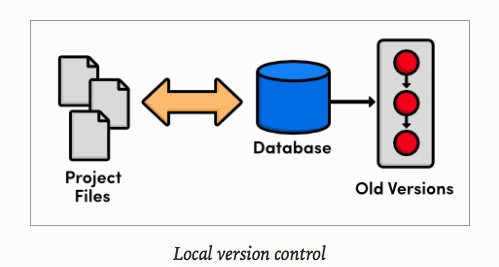
\includegraphics[width=3.5cm]{images/grafico5.png}	 %importamos una imagen
%	\caption{ descripcion de la imagen}
%\end{minipage}
%\end{figure}

\subsection{Model}
En este Paquete se encuentrar los modulos encargados de la manipulacion de datos de nuestro software.\\
Como estructura de almacenamiento tomamos a las estructuras XML, ya que nos permite guardar y acceder a su informacion de un manera muy sencilla, y dada su portablilidad podemos acceder a ella desde cualquier ruta en la que este alojada.\\

Este paquete cuenta con las siguientes clases y datos :
\begin{itemize}
	\item \textbf{Data.- }Clase que extiende de la clase etree.Element que nos permitira manipular datos de estructuras de tipo XML.
	
	La estructura XML es la siguiente:
	\begin{itemize}
		
	 \item \textbf{Objeto datos.- }Objeto que almacena el punto de partida desde que se empezo a grabar el movimiento del robot
	 
	 \item \textbf{Objeto movimiento.-}Objeto que almacena datos acerca de un movimiento grabado, tiene los siguiente atributos:
	 	\begin{itemize}
			\item \textbf{tiempo.- }Atributo que contiene un timer en milisegundos que es tiempo que se ejecuto un movimiento "X"
			
			\item \textbf{movimiento.- }Atributo que contiene el tipo de movimiento que se hiso, ya se que avanzo, se detuvo o si giro.
			
			El valor de este atributo dependera de la Clase Evento, puesto que esta es la que maneja los eventos de teclado, y cada evento esta relacionado a una accion, es aqui donde se puede apreciar, ya que este atributo representa una accion que realizo la clase Evento.
			
			\item \textbf{pinza.- }Atributo que contiene el estado de si pinza, es decir si este la tiene abierta o cerrada "T", si esta abierta y "N en caso contrario".
			
		\end{itemize}
	\end{itemize}
	\item \textbf{Estadistica.- }Clase la cual nos proporciona datos estadisticos del robot, desde que se inicio el programa, como ser cuantos movimiento hiso, cuales fueron los movimentos que mas se realizo, ..etc


\end{itemize}

	

\section{ALGORITMIA}
Un problema que se tuvo fue la lectura y escritura de los datos al momento de grabar y reproducir el movimiento del robot. Esto de dio ya que se estaba almacenando los estados de los movimiento del robot cada cierto intervalo de tiempo "X" , lo cual implicaba que la escrituta de los datos fuera bastante.\\

Un ejemplo fue que se grababa los estados del robot cada 100 milisegundos, por lo cual si queriamos grabar 5 minutos de movimientos, implicaria escribir 3000 movimientos.A esto aumentar que si queriamos movimentos mas exactos habria que reducir el intervalor de tiempo, lo cual implica mas datos y mas propenso a perder los mismo.\\

Tambien como contabamos con varios datos esto constituia un gran uso de la memoria RAM para reproducir todos estos movimiento, y sobre esto agregar que la conexion al arduino por el puerto serial es Asincrona, lo cual implica que si perdiamos un dato o varios de estos, nuestra grafica ya no sera tan exacta como esperamos.\\

Acontinuacion se muestra los algoritmos mensionados:\\

\begin{algorithm}[H]
	\SetKwData{Left}{left}\SetKwData{This}{this}\SetKwData{Up}{up}
	\SetKwFunction{Union}{Union}\SetKwFunction{FindCompress}{FindCompress}
	\SetKwInOut{Input}{input}\SetKwInOut{Output}{output}
	%%\Input{root of a file XML}
	%%\Output{file XML with the data of robot movements  }
	\BlankLine
	Open file XML;\\
	\While{is recording}{
		write movements;\\	
		sleep(100);
	}
	close file XML;\\
	\caption{Algorithm to store robot movements }
\end{algorithm}

\begin{algorithm}[H]
	\SetKwData{Left}{left}\SetKwData{This}{this}\SetKwData{Up}{up}
	\SetKwFunction{Union}{Union}\SetKwFunction{FindCompress}{FindCompress}
	\SetKwInOut{Input}{input}\SetKwInOut{Output}{output}
	%%\Input{root of a file XML}
	%%\Output{play robot movements}
	\BlankLine
	Open file XML;\\
	\While{there is data}{
		data = read movements;\\
		reproduce( data );\\
		sleep(100);
	}
	close file XML;\\
	\caption{Algorithm to reproduce robot movements }
\end{algorithm}

Para solucionar este problema, puesto que nuestro algoritmo no era eficiente y menos eficaz, se implemento el siguiente algoritmo que acoparacion del anterior, este no guarda datos en cada intervalo de tiempo, sino que guarda datos cada vez que se detecta cambios en el robot, es decir que si se detecta un cambio de estado en el robot, como ser girar, mover,abrir o cerrar pinza, este guarda el tiempo que tarda en realizar esta accion, de esta manera optimizamos los recursos de nuestro computador(Eficiencia Temporal) como ser memoria(RAM), puesto que ya no tiene que leer datos cada cierto intervalo de tiempo sino que cuando sea necesario  y ademas tenemos movimientos mas exactos, puesto que reducimos la perdida de datos al momento de reproducirlo , ya que trabajamos con tiempos de reloj y no asi con intervalos.

Acontinuacion se muestra el algoritmo mensionado:\\

\begin{algorithm}[H]
	\SetKwData{Left}{left}\SetKwData{This}{this}\SetKwData{Up}{up}
	\SetKwFunction{Union}{Union}\SetKwFunction{FindCompress}{FindCompress}
	\SetKwInOut{Input}{input}\SetKwInOut{Output}{output}
	\Input{root of a file XML}
	\Output{file XML with the data of robot movements  }
	\BlankLine
	open file XML;\\
	write initial data;\\	
	\While{is recording}{
		\uIf{is firts iteraction}{
			time = get Time Of Computer;\\
			lastMovement = Robot movement ;
		}
		\uElseIf{was a change in the robot}{
			time = get Time Of Computer - time;\\
			write lastMovement and time;\\
			lastMovement = Robot movement;			
		}
	}
	
	close file XML;\\
	\caption{New algorithm to store robot movements }
\end{algorithm}


\begin{algorithm}[H]
	\SetKwData{Left}{left}\SetKwData{This}{this}\SetKwData{Up}{up}
	\SetKwFunction{Union}{Union}\SetKwFunction{FindCompress}{FindCompress}
	\SetKwInOut{Input}{input}\SetKwInOut{Output}{output}
	\Input{root of a file XML}
	\Output{play robot movements}
	\BlankLine
	Open file XML;\\
	read initial data;\\ 
	\While{there is data}{
		data = read movements;\\
		time = read time;\\
		reproduce( data, time  );\\
	}
	close file XML;\\
	\caption{New algorithm to reproduce robot movements }
\end{algorithm}


\section{METODOLÓGICA Y FUENTE}


Las fuente de información que tomamos como base para desarrollar el proyecto son principalmente publicas y bibliográficas\\

Tambien para el desarrolo del proyecto se trabajo con la metodologia agil Scrum, puesto que era la que mas se adaptaba mas a nuestra comodidad.\\



Como Sistema de Control de Versiones se uso GitHub, ya que nos permite el trabajo colaborativo y no presencial(\url{https://github.com/akey96/TallerDeProgramacion}\\)


Para el desarrollo de la documentacion se uso el formato ACM.

\subsection{Composicion de grupo}

Esta parte falta definir, puesto que recien implementaremos modulos faltantes.................


%\section{CONCLUSIONES}

%\subsection{Resultados del desarrollo del proyecto}

%a que hemos llegado con esta investigacion y que podemos destacar de esta y problemas con los cuales nos topamos....
\newpage
\section{GLOSARIO DE TÉRMINOS}
\subsection{Diccionario}
\begin{itemize}
	
	\item \textbf{Arduino.- } Arduino es una plataforma de prototipos electrónica de código abierto (open – source) basada en hardware y software flexibles y  fáciles de usar. Está pensado e inspirado en artistas, diseñadores, y estudiantes de computación o robótica
	
	\item \textbf{Concurrecia.- } evento cuando  mas de un proceso intentan acceder al mismo recurso 
	
	\item \textbf{MVC .- }Arquitectura de software que separa los datos de una aplicación, la interfaz de usuario, y la lógica de control en tres componentes distintos.
	
	\item \textbf{Singleton.- } Es un patrón de diseño que permite restringir la creación de objetos pertenecientes a una clase o el valor de un tipo a un único objeto.Su intención consiste en garantizar que una clase solo tenga una instancia y proporcionar un punto de acceso global a ella.
	
	\item \textbf{Eficiencia Espacial.- }Cantidad de recursos espaciales ( de  almacén) que un algoritmo consume o necesita para su 
	ejecución
	
	\item \textbf{SCV.- }  Software que administra el acceso a un conjunto de ficheros, y mantiene un historial de cambios realizados. El control de versiones es útil para guardar cualquier documento que cambie con frecuencia, como código fuente, documentación o ficheros de configuración.
	
	\item \textbf{XML.- } XML proviene de eXtensible Markup Language (“Lenguaje de Marcas Extensible”). Se trata de un metalenguaje (un lenguaje que se utiliza para decir algo acerca de otro) extensible de etiquetas que fue desarrollado por el Word Wide Web Consortium (W3C)
	
	\item \textbf{Comunicacion Asincrona.- }Es la conexión que se establece entre el cliente y el servidor que permite la transferencia de datos no sincrónica, o sea el cliente puede realizar varias peticiones al servidor sin necesidad de esperar por la respuesta de la primera. 
	
		
\end{itemize}

\newpage


\section{BLIBLIOGRAFIA}

%\renewcommand\refname{Bibliografía}

\begin{thebibliography}{9}
%\bibitem(Vesperman,2007){Vesperman} J. Vesperman. “Essential CVS”. O’Really Media Inc, 2007.
\bibitem{Singleton}{mundoerp} http://mundoerp.com/blog/Singleton
\bibitem{Arduino}{arduinodhtics} https://arduinodhtics.weebly.com/iquestqueacute-es.html
\bibitem{xml}{definicion} https://definicion.de/xml/
\bibitem{Comunicacion Asincrona}{ecured} https://www.ecured.cu/Comunicaci\%C3\%B3n\_as\%C3\%ADncrona
\bibitem{SCV}{mundoerp} http://mundoerp.com/blog/sistemas-de-control-de-versiones/
\end{thebibliography}

\newpage

\end{document}

